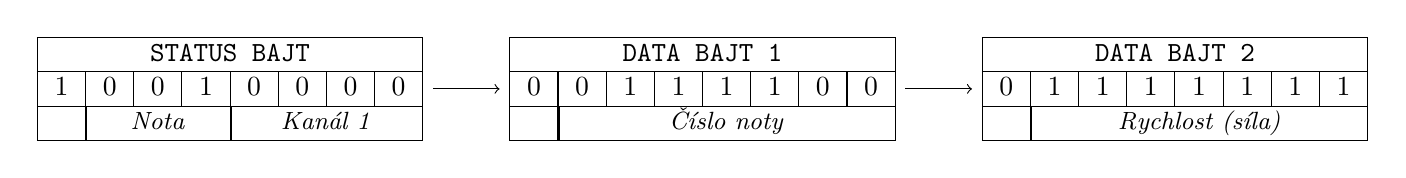
\begin{tikzpicture}[]
\draw (0,0) node (stab) { 
    \begin{tabular}{|c|c|c|c|c|c|c|c|}
        \hline
        \multicolumn{8}{|c|}{\texttt{STATUS BAJT}} \\
        \hline
        1 & 0 & 0 & 1 & 0 & 0 & 0 & 0 \\
        \hline
         &  \multicolumn{3}{|c|}{\small\emph{\uv{Nota}}} & \multicolumn{4}{|c|}{\small\emph{Kanál 1}} \\
        
        \hline
    \end{tabular}
};

\draw (6,0) node (datb1){
    \begin{tabular}{|c|c|c|c|c|c|c|c|}
        \hline
        \multicolumn{8}{|c|}{\texttt{DATA BAJT 1}} \\
        \hline
        0 & 0 & 1 & 1 & 1 & 1 & 0 & 0 \\ 
        \hline
        &  \multicolumn{7}{|c|}{\small\emph{Číslo noty}} \\
        
        \hline
    \end{tabular}
};

\draw (12,0) node (datb2){
    \begin{tabular}{|c|c|c|c|c|c|c|c|}
        \hline
        \multicolumn{8}{|c|}{\texttt{DATA BAJT 2}} \\
        \hline
        0 & 1 & 1 & 1 & 1 & 1 & 1 & 1 \\ 
        \hline
        &  \multicolumn{7}{|c|}{\small\emph{Rychlost (síla)}} \\
        
        \hline
    \end{tabular}
};

\draw[->] (stab.east) -- (datb1.west);
\draw[->] (datb1.east) -- (datb2.west);
\end{tikzpicture}


